%%This chapter is used to show our implementation in ProM.  It can be split into 3 parts. 
%The first one is the Dfg method, including the weight update, process tree generation and petri net without long-term dependency generation.
% The second part is to add long-term dependency, it can be use as whole part or customized part into model, also removing the long-term dependency
% Evaluation part is the confusion matrix measurement.
ProM is an open-source extensible framework. It supports wide process mining techniques in the form of plug-ins\cite{ProM}. The algorithm to incorporate negative information is implemented as one plug-in called \textbf{\emph{Repair Model By Kefang}} in ProM and released online\cite{MyPlugin}. This chapter is divided into four parts to describe the whole implementation. Firstly, the inputs and outputs of this implementation is introduced. After accepting the inputs, a directly-follows graph is constructed by dfg-method and later converted into process tree or Petri net process model. Next, the implementation to add long-term dependency on the process model from last step is shown. At last, another feature is displayed to show the brief evaluation result based on confusion matrix. 
\section{Inputs And Outputs}
The plug-in inputs are an event log $L$ with labels to classify each trace and an existing model N possible in multiple forms.
\begin{itemize}
	\item Acceptable event log L with labels. Labels are one trace attribute and used to identify the positive and negative instances. 
	\item Acceptable Process Models
	\begin{itemize}
		\item Petri net + Initial Marking.
		\item Accepting Petri net. \\
		The initial marking is already included into the accepting Petri net. 
		\item Petri net.\\ In this situation, the initial marking is guessed automatically in the background program.
	\end{itemize}
\end{itemize}

The outputs are one process model and its corresponding initial marking. They are exported from the control panel in the result view and can be in various forms.
\begin{itemize}
	\item Petri net with long-term dependency after Reducing Silent Transition
	\item Petri net with long-term dependency
	\item Petri net without long-term dependency
	\item Process tree
\end{itemize}

\section{Implementation of dfg-method }
Firstly the dialog for options to generate directly-follows graphs from event log pops up. Event classifier are set by those dialogs. Subsequently, a dialog is shown to set the Inductive Miner parameters. The parameters include the Inductive Miner variant and the noise threshold to filter the data. The dialog is displayed in Figure \ref{fig:dfg-IM-setting}.
\begin{figure}
	\centering
	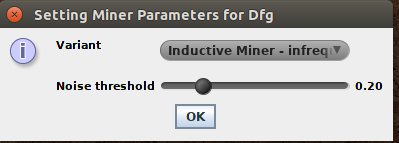
\includegraphics[scale=0.75]{figures/implementation/dfg-IM-setting.png}
	\caption{Inductive Miner Parameter Setting}
	\label{fig:dfg-IM-setting}
\end{figure} \\
After setting the parameters, process models  of process tree and Petri net without long-term dependency can be generated by Inductive Miner and displayed in the result view in Figure \ref{fig:dfg-IM-pn-without-lt}. 
\begin{figure}
	\centering
	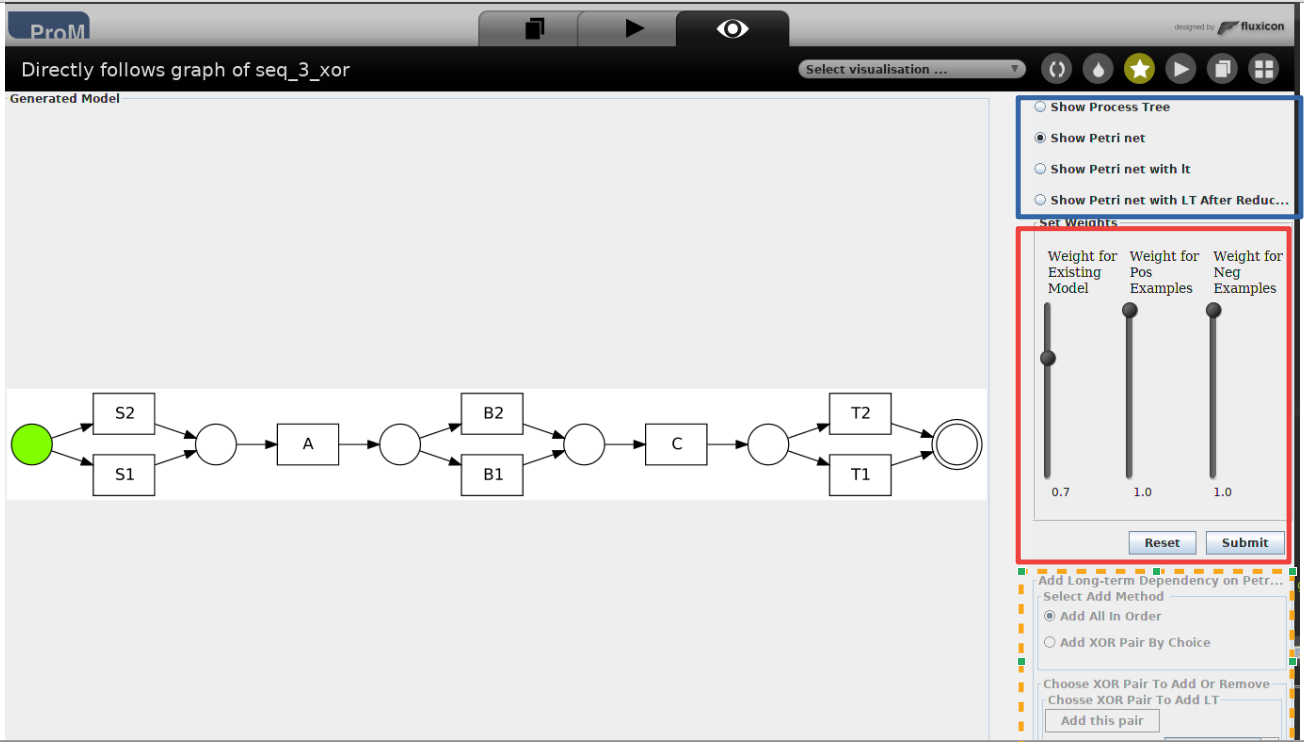
\includegraphics[width=\textwidth]{figures/implementation/dfg-IM-pn-without-lt.png}
	\caption{Generated Petri net without long-term dependency}
	\label{fig:dfg-IM-pn-without-lt}
\end{figure}
The left side is the model display area. To allow more flexibility, this plug-in are interactive by the control panel, which is the right side of result view. Originally, only the generated model type and the weight sliders are enabled, while the control panel for adding long-term dependency are invisible. 

The model type are in the blue rectangle marked in Figure \ref{fig:dfg-IM-pn-without-lt}. It has 4 options to control the generated model type. Currently, the option "Show Petri net" is chosen, so the constructed model is Petri net without long-term dependency. The weights sliders are in red rectangle. It enables to adjust the weights on the existing model, positive and negative instances. Once submitted those options, different process models are mined under different weights. The rectangle in orange are the invisible part to control long-term dependency options. It is discussed in the next section.

\section{Implementation of Adding Long-term Dependency }
If the model ro generate is Petri net with long-term dependency, the program to add long-term dependency is triggered. This program in the background detects and puts places and silent transitions on Petri net directly mined from Inductive Miner to add long-term dependency. As comparison, the same weight setting is kept like the Figure \ref{fig:dfg-IM-pn-without-lt}, but the option to show a Petri net with long-term dependency is chosen. The resulted model is Figure \ref{fig:dfg-IM-pn-with-lt}. 
\begin{figure}
	\centering
	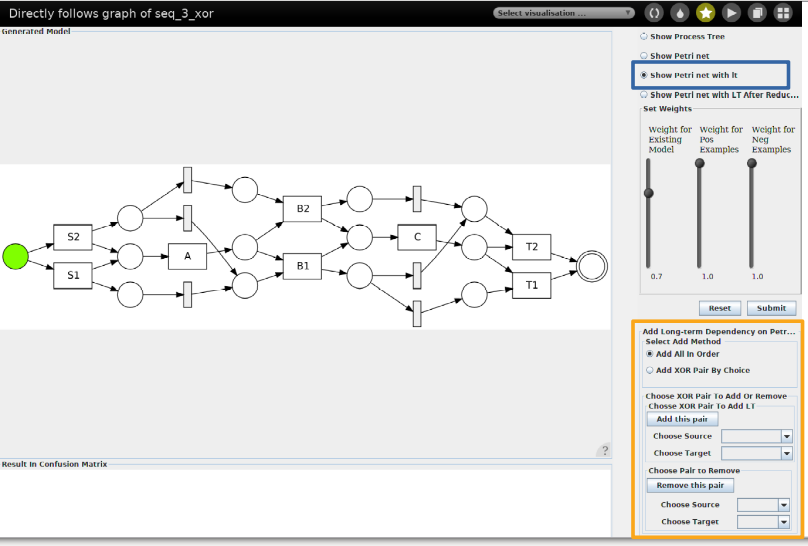
\includegraphics[width=\textwidth]{figures/implementation/dfg-IM-pn-with-lt.png}
	\caption{Petri Net with long-term dependency }
	\label{fig:dfg-IM-pn-with-lt}
\end{figure}

Meanwhile, the control part of adding long-term dependency turns visible, which is in the orange rectangle in Figure \ref{fig:dfg-IM-pn-with-lt}.  It has two main options, one is to consider all long-term dependency existing in the model, the other is to choose the part manually. It allows more flexibility for users. Below those two options, it is the manual selection panels, including control part to add and remove pair. As an example, the blocks Xor(S1,S2) and Xor(T1,T2) are chosen to add long-term dependency. It results in the model in Figure \ref{fig:dfg-IM-pn-with-lt-m}. 
\begin{figure}
	\centering
	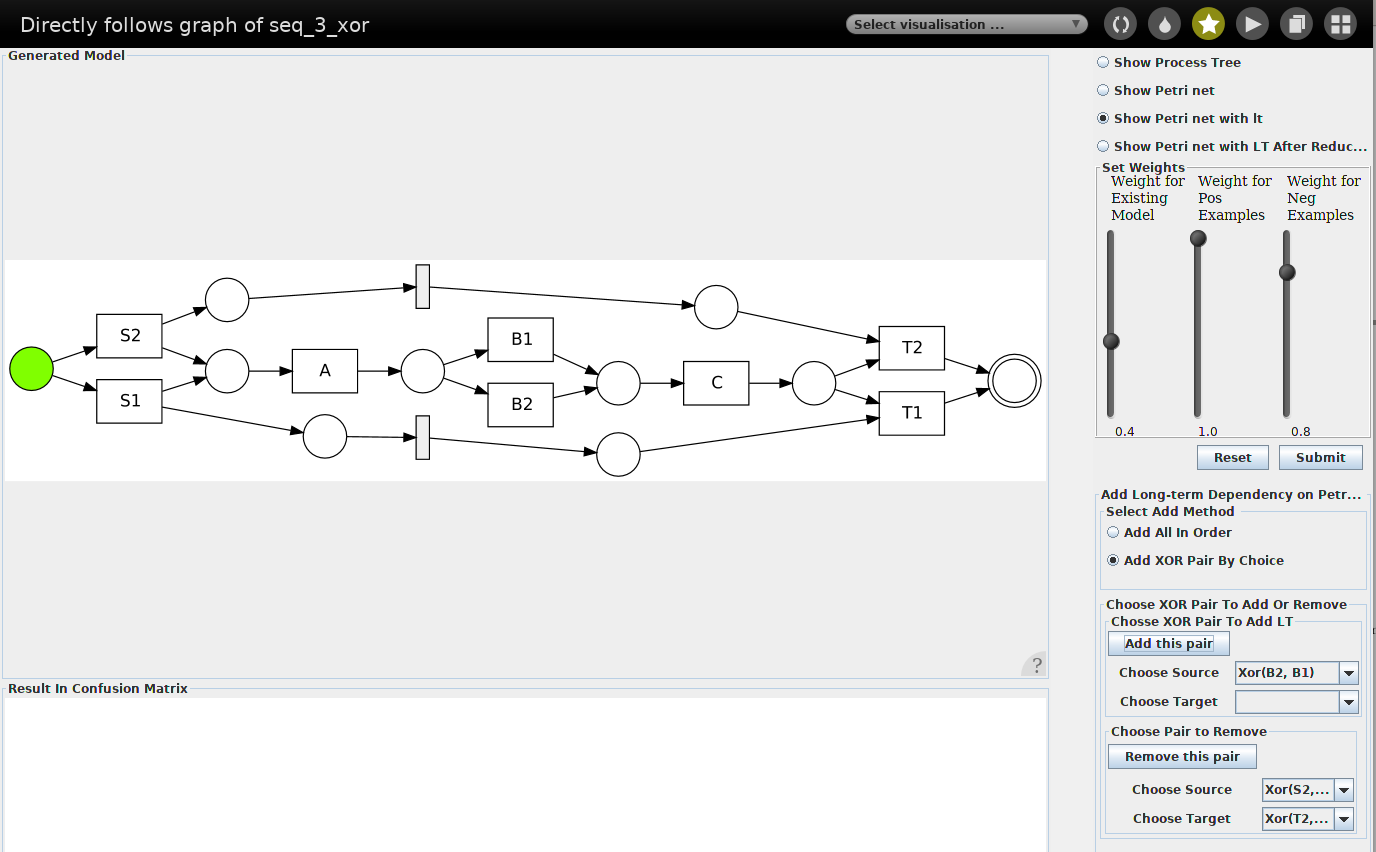
\includegraphics[width=\textwidth]{figures/implementation/dfg-IM-pn-with-lt-manual.png}
	\caption{Petri net with selected long-term dependency}
	\label{fig:dfg-IM-pn-with-lt-m}
\end{figure}

By choosing \emph{Petri net with LT After Reducing} in model type option panel, silent transitions are reduced to simplify the model.
Under the same setting in Figure \ref{fig:dfg-IM-pn-without-lt}, the simpler model in Figure \ref{fig:dfg-IM-pn-with-lt-r} is constructed, after the post processing of reducing silent transitions.
\begin{figure}
	\centering
	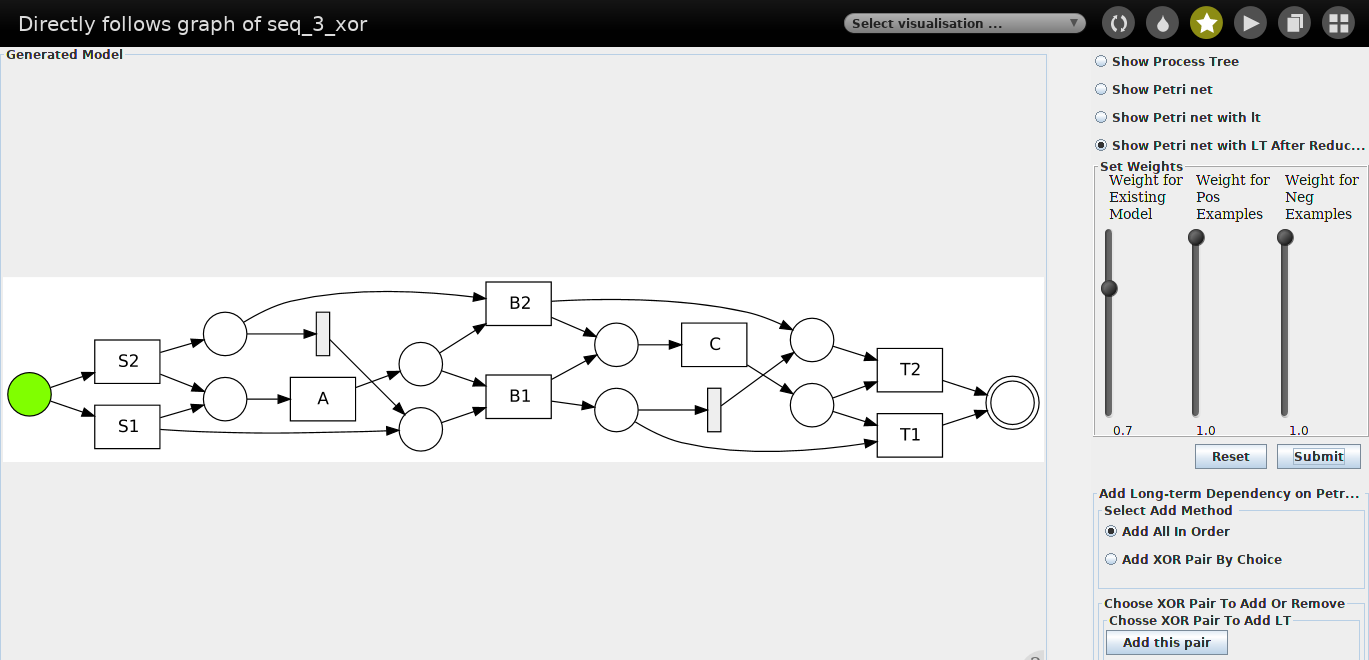
\includegraphics[width=\textwidth]{figures/implementation/dfg-IM-pn-with-lt-reduced.png}
	\caption{Petri net after reducing the silent transitions}
	\label{fig:dfg-IM-pn-with-lt-r}
\end{figure}

\section{Implementation of Showing Evaluation Result}
Another feature in this plugin  is to show the evaluation result based on confusion matrix. With the brief evaluation result, it helps set the parameter and select the final process model. 

It works in this way. After creating the current model in the left view, the evaluation program in background uses the event log and the current Petri net in the view as inputs. It applies a naive fitness checking and generates a confusion matrix with relative measurements like recall, precision. This evaluation result is then shown in the bottom of the left view in Figure \ref{fig:dfg-IM-cm}.  If the button of green rectangle in the right view \emph{Show Confusion Matrix} is pressed again, the program is triggered again and generates a new  confusion matrix result in  dark green dashed rectangle which will be listed above the previous result in light green dashes area. 
\begin{figure}
	\centering
	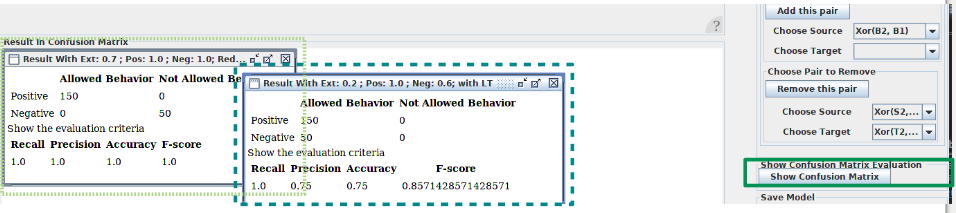
\includegraphics[width=\textwidth]{figures/implementation/dfg-IM-confusionmatrix.png}
	\caption{Generated Process Tree Model}
	\label{fig:dfg-IM-cm}
\end{figure}

